
We start our analysis by quantifying the consequences of a deviance from the flows' balance on the underlying marginal distribution over the terminal states. Our results highlight, on the one hand, that a lack of flow-balance upstream in the generative process is more damaging to the overall distributional accuracy of a GFlowNet than an equivalent imbalance nearer the terminal states; on the other hand, that a disruption of the detailed balance condition in a single edge may be catastrophically propagated within the network and severely damage the approximation to the target distribution. See the appendix for self-contained proofs of our results. 

\begin{figure}[t]
    \center 
    \def\spacing{-15pt}
\[\begin{tikzcd}
	&[\spacing]&[\spacing] {F+\delta} \\
	&[\spacing] {\frac{F}{g}+\delta} &[\spacing]&[\spacing]&[\spacing] {\frac{F}{g}} \\
% 	& \triangle & \triangle && \triangle & \triangle \\
    {\frac{F}{g^h}+\delta_1} &[\spacing] {\frac{F}{g^h}+\delta_2} &[\spacing]&[\spacing] % {\frac{F}{g^h}+\delta_{g^{h-1}}} 
    &[\spacing] {\frac{F}{g^h}} &[\spacing] {\frac{F}{g^h}} % & {\frac{F}{g^h}}
    \arrow["{\text{degree g}}", swap, from=1-3, to=2-2]
	\arrow[from=1-3, to=2-5]
	\arrow[from=2-5, to=3-6]
	\arrow[from=2-5, to=3-5]
	\arrow[from=2-2, to=3-1]
	\arrow[from=2-2, to=3-2] 
    % \arrow[from=3-2, to=4-1]
	% \arrow[from=3-2, to=4-2]
	% \arrow[from=3-3, to=4-3]
	% \arrow[from=3-5, to=4-5]
	% \arrow[from=3-6, to=4-6]
	% \arrow[from=3-6, to=4-7]
\end{tikzcd}\]
\caption{\textbf{Imbalanced flows in a regular tree} with width $g = 2$ and depth $h = 2$. The extra flow within the root's left child breaks the expected uniform distribution over the $g^{h}$ leaves.}
% \caption{\textbf{Imbalanced flow network in a tree.}}
% \caption{A flow network with a extra flow of $\delta$ in one of the branches of the initial state} 
    \label{fig:a} 
    % \label{fig:treesgraphs} 
\end{figure}

% \begin{theorem}[Total variation of the sampling distribution] Let $\delta >0$ and $\sum_{i=1}^{g^{h-1}} \delta_i = \delta$, where $\delta_i \in [0, \delta]$ for all $i \in \{1,2, \dots, g^{h-1}\}$. Suppose that we have the flow network $(G_T, F+\delta)$ abiding by Assumption~\ref{as: gf_tree_unif} besides the first edge from the root to a son where it has a $\delta$ increasing generating a new target distribution $\pi$ (see Figure [ref]).  Under these conditions, the total variation distance between $\pi$ and $\pi^*$ is bounded above and below by 
% \begin{align*}
% & \epsilon(\delta, g) \leq ||\pi - \pi^*||_{\scaleto{\textbf{TV}}{3pt}} \leq \epsilon(\delta, g^h) \quad \text{where}
% \\
% & \epsilon(a,b) := \Big(1 - \frac{1}{b} \Big) \frac{a}{F+a}\,.
% \end{align*}
% \end{theorem}


\vspace{4pt}\noindent\textbf{Bounds on TV for arbitrary state graphs.} We show that the intuition built upon the previous discussion relatively to tree-structured state graphs carries out to general acyclic generative processes, namely, (i) that an imbalanced edge reaching many terminal states has a larger impact on the approximation to the target distribution than an imbalanced edge leading to comparably fewer terminal states; and (ii) the difficult of training a GFlowNet is an increasing function of the target distribution's support. To start with, \autoref{thm:wca} lays out a worst-case analysis of the propagated errors within a flow network and underlines point (ii) above. 

\begin{theorem}[Deterministic flow-based bounds for the TV in general graphs] \label{thm:wca} 
    Let $(\mathcal{G}, F, \tilde{\pi})$ be a imbalanced flow network defined on a DAG $\mathcal{G}$ and $\tilde{\pi}$ be an uniform distribution supported on a space with $n$ objects. Assume that, except for an edge $(u, v)$ in $\mathcal{G}$, i.e., $\mathbf{A}_{uv} = 1$, for which  
    \begin{equation}
        F(s) p_{F}(s, s') - F(s') p_{B}(s', s) = \delta 
    \end{equation}
    with $\delta \ge 0$, the network is balanced. Let $p_{\intercal}^{(\delta)}$ be the corresponding marginal distribution over $\mathcal{X}$ and $d$ be the number of reachable terminal states from state $v$. Then, 
    \begin{equation}
        \frac{\delta (n - d)}{2n (F + \delta)} \le \|p_{\intercal}^{(\delta)} - \pi\|_{\scaleto{\textbf{TV}}{3pt}} \le \frac{\delta (n - 1)}{2n (F + \delta)}, 
    \end{equation}
    in which $\pi \propto \tilde{\pi}$ and $F(s_{o}) = F + \delta$ is the total flow. 
\end{theorem}
% \begin{theorem}[Total variation of the sampling distribution] Let $(G_n, F)$ be a flow network which should generates a target distribution $\pi$ uniform in the number of final vertices. Suppose there exists an edge in $G_n$, that is $s \to s' \in \mathbb{A}$ such that
% \[  F(s)P_{F}(s' | s) - F(s')P_{B}(s|s') = \delta \,,\]
% where $\delta > 0$. Then we have that $(G_n, F)$ generates a probability distribution $\mu_{\delta}$ such that
% \begin{align*}
% & \frac{\delta(n - d)}{2n(F + \delta)} \le ||\mu_{\delta} -\pi||_{\scaleto{\textbf{TV}}{3pt}} \leq \frac{\delta(n + dn - d)}{2n(F + \delta)} \,,
% \end{align*}
% where $d \in \{1,2, \dots, n-1\}$ is the number of final vertices that are descendants of $s'$. 
% \end{theorem}

Remarkably, this result shows that the accuracy of the downstream distribution depends linearly upon the deviation from the detailed balance within a single edge and, therefore, even a small error may lead to significant disruptions in the distributional approximation. Correspondingly, the result underscores the hardening properties of the number $n$ of terminal states regarding the training of GFlowNets: both the (provably tight) lower and upper bounds are increasing functions of $n$. Nonetheless, the preceding statement is poorly informative about the relevance of the particular imbalanced state to the overall generative process, an often observed phenomenon in worst-case analyses. In this context, we show in \autoref{thm:random} that, assuming Dirichlet-distributed downstream flows $\delta_{1}, \dots, \delta_{d}$ as shown in \autoref{fig:a} and an uniform target, the average TV distance between the learned and target distributions is an increasing function of the number of reachable states from the imbalanced node.  

\begin{theorem}[Expected TV under Dirichlet-distributed extra flows]\label{thm:random} 
    Let $(\mathcal{G}, F, \tilde{\pi})$ be the same imbalanced flow network as in \autoref{thm:wca}. Assume that the extra flow $\delta$ is distributed among the imbalanced node's terminal children according to a Dirichlet distribution with concentration parameter $\alpha \in \mathbb{R}^{d}$, i.e., 
    \begin{equation*}
        \left(\nicefrac{\delta_{i}}{\delta}\right)_{1 \le i \le d} \sim \textrm{Dir}\left(\alpha\right) % .   
    \end{equation*}
    (see \autoref{fig:a} for an illustration in trees). Denote $x_{i} = \nicefrac{\delta_{i}}{\delta} \in [0, 1]$ for $1 \le i \le d$ and $\mu_{\mathbf{x}, \delta}$ for the distribution resulted from the corresponding $\delta$-imbalance. Then, 
    \begin{equation*}
        \underset{\mathbf{x} \sim \textrm{Dir}(\alpha)}{\mathbb{E}} \left[ \|\mu_{\mathbf{x}, \delta} - \pi\|_{TV} \right] = \left( d \left( \Lambda - \frac{1}{n} \right) + 1 \right) \cdot \frac{\delta}{2(F + \delta)}, % .   
    \end{equation*}
    with, by letting $F_{a,  b}$ be the CDF of a $\textrm{Beta}(a, b)$ distribution,  
    \begin{equation*}
        \Lambda = \nicefrac{2}{n} F_{\alpha_{i}, 2\bar{\alpha}_{i}} \left( \nicefrac{1}{n} \right) - 2 F_{\alpha_{i} + 1, 2\bar{\alpha}_{i} + 1} \left( \nicefrac{1}{n} \right) + 1 - \nicefrac{1}{n} % . 
    \end{equation*}
    and $\bar{\alpha}_{i} = \sum_{j \neq i} \alpha_{j}$. 
\end{theorem}

However, it is unclear whether $\Lambda > \nicefrac{1}{n}$ and, in particular, whether $d$ positively or negatively influences the expected TV distance: for $n = 1$, $\Lambda = 0$, whereas $\lim_{n \rightarrow \infty} \Lambda = 1$. In this sense, \autoref{thm:random}'s corollary below reveals that, for uniformly distributed $\delta_{i}$, $d$ has a positive effect on the expected approximation error in all practically relevant cases, reiterating that ensuring the flow-balance in nodes from which many terminal states are reachable must be prioritized during training --- as we previously remarked in the context of tree-based state graphs. 

\begin{corollary} \label{col:random} 
    In \autoref{thm:random}, let $\alpha_{i} = 1$ for each $1 \le i \le d$, i.e., $(\nicefrac{\delta_{i}}{\delta})_{i=1}^{d}$ is uniformly distributed within the $(d + 1)$-dimensional simplex. Under these conditions, 
    \begin{equation*}
        \Lambda(d, n) = (d - 1) \left( \frac{1}{2} - \frac{1}{n} + \frac{1}{n^{2}}\right)  
    \end{equation*}
    and the expected TV between $\mu_{\mathbf{x}, \delta}$  and $\tilde{\pi}$, 
    \begin{equation*}
        \frac{\delta}{2(F + \delta)} \left( d \left( \Lambda(d, n) - \frac{1}{n} \right) + 1 \right),   
    \end{equation*}
    is an increasing function of $d \ge 1$ for $n > 2$. 
\end{corollary}
% Remarkably, this is very and very threatening to mankind and to the planet.  

% This is a weighted version of the detailed balance condition, which may be adequate for large state spaces under constraining computational settings

% \vspace{4pt}\noindent\textbf{Transition-decomposable and discriminatory DB loss ($\text{TD}^{3}$).}  

\vspace{4pt}\noindent\textbf{Theoretical analysis for tree-structured state graphs.} To gain some intuition, we first consider the scenario in which the state graph $\mathcal{G}$ is a regular tree with depth of $h$ in which each node, except the leaves representing the terminal states, has $g$ children and that the target distribution is uniform; see \autoref{fig:a}. Under these conditions, \autoref{thm:a} underscores that an improperly estimated flow near the initial state may significantly hinder the distributional approximation. 

\begin{example}[Total variation of the sampling distribution for trees] \label{thm:a} 
    Let $(\mathcal{G}, F, \tilde{\pi})$ be a balanced flow network with state graph $\mathcal{G}$ that is a tree with width $g$ and depth $h$, flow $F$ and uniform target distribution $\tilde{\pi}$.  Define $\delta \ge 0$ and $\sum_{i=1}^{g^{h - 1}} \delta_{i} = \delta$, with $\delta_{i} \in [0, \delta]$ for all $i \in \{1, 2, \dots, g^{h - 1}\}$. Then, assume that the flow within an edge stemming from the root has an increase of $\delta$, leading to an non-uniform marginal distribution $p_{\intercal}$ over the leaves; see \autoref{fig:a}. In this scenario, the total variation distance between $p^{\intercal}$ and $\pi \propto \tilde{\pi}$ is bounded above and below by 
    \begin{equation}
    \label{eq:a} 
    \begin{aligned}
        \epsilon(\delta, g, F) \leq \|p_{\intercal} - \pi\|_{\scaleto{\textbf{TV}}{3pt}} \leq \epsilon(\delta, g^{h}, F), \, \text{with } 
        \epsilon(\delta, x, F) \coloneqq \left(1 - \frac{1}{x}\right) \frac{\delta}{F + \delta}.  
    \end{aligned}
    \end{equation} 
\end{example}

Notably, \autoref{eq:a} reveals that the effect of a broken balance of the learned flows over the downstream distribution crucially depends upon the height $h$ and, particularly, of the number of reachable leaves from the imbalanced edge; that is, the upper bound on the TV distance between $p_{\intercal}$ and $\pi$ increases exponentially in $h$ through $g^{h}$. Likewise, the lower bound on the TV increases as a function of the tree's width $g$, implying that the impact of the imbalance of the flows over $p_{\intercal}$ is larger for large state graphs than for comparably small ones. This underlines the advantages of building parsimonious state graphs and rigorously explains why the difficult of training a GFlowNet increases as we endeavor to approximate distributions with larger supports. 

\vspace{4pt}\noindent\textbf{Going beyond uniform distributions.} Our analysis was up to this moment based on the assumption of an uniform target distribution. Although insightful, this approach is somewhat constraining since a practitioner is generally interested in sampling from non-uniform distributions. In this context, \autoref{thm:app:a} in the appendix extends the previous results to multi-modal distributions and shows, similarly to \autoref{thm:a}, the relevance of upstream states and, differently from prior discussion, that the impact on the distributional accuracy of a lack of balance at a state having a large amount of probability mass concentrated among its descendants is larger than the impact corresponding to the imbalance of a state associated to a relatively small probability mass. This justifies, e.g., the empirical success of the replay buffer, which stores trajectories leading to high-probability terminal states and periodically replays them during training to reduce their associated error. 

% \vspace{4pt}\noindent\textbf{Transition-decomposable and discriminatory DB loss ($\text{TD}^{3}$).} 
\vspace{4pt}\noindent\textbf{Transition-decomposable discriminatory DB loss ($\text{TD}^{3}$).} \autoref{thm:a}, \autoref{thm:wca} and \autoref{thm:random} emphasized under different circumstances that, during training, one should prioritize ensuring the flow balance of states that are ancestral to high probability regions of the target distribution. Hence, we build upon this fact to define, for a trajectory $\tau = (s_{o}, s_{1}, \dots, s_{m})$, the loss function 
\begin{equation*}
    \mathcal{L}_{TD}(\tau) = \frac{1}{\sum_{i} \gamma(s_{i})} \sum_{1 \le i \le m} \gamma(s_{i}) \mathcal{L}_{i - 1, i}(\tau)% , 
\end{equation*}
(see \autoref{eq:stbalance}), in which $s \mapsto \gamma(s)$ is a weighting function; we call $\mathcal{L}_{TD}$ the \textit{transition-decomposable discriminatory detailed balance loss} ($\text{TD}^{3}$). Ideally, $\gamma(s)$ would be proportional to the probability mass associated with the $s$'s terminal descendants. In practice, however, it is very difficult to estimate such quantity in general state graphs and we instead consider $\gamma(s) = (T - d(s, s_{o}))^{2}$ as a proxy to this quantity, with $d(s, s_{o})$ as the geodesic distance between $s$ and the state graph's initial state and $T$ as the maximum trajectory length, which is always known. Intuitively, $\gamma$ assigns high weight to nodes upstream in the generative process leading to a large number of terminal states and, thus, related to a high probability region of the target. Moreover, we regard $\gamma$ as a quadratic function of $d(s, s_{o})$ (instead of a linear one) for the expected TV in \autoref{col:random} quadratically depends upon the imbalanced node's terminal children.   

% Moreover, we regard $\gamma$ as a quadratic function of $d(s, s_{o})$ as the expected TV in \autoref{col:random} quadratically depends upon the node's children.    

% Moreover, we regard $\gamma$ as a quadratic function of $d(s, s_{o})$ due to the quadratic dependence 

% Write about the annealing stuff (in the empirical section) and about using square instead of linear weighting 

\begin{figure}[!t] 
    \centering
    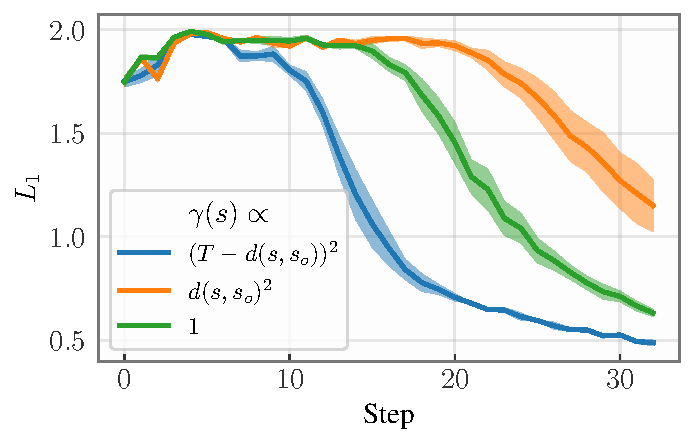
\includegraphics[width=.45\linewidth]{figures/avg_l1_gflownets_sets_weighted_db.pdf}
    \caption{\textbf{Weighted DB accelerates training convergence relatively to standard DB.} By weighting each transition proportionally to its closeness to the state graph's root, we notoriously improve upon the DB loss. This empirically supports our theoretical claims regarding the elevated importance of ensuring the balance within states leading to a large number of terminal states.}
    \label{fig:aaa}
\end{figure}

\vspace{4pt}\noindent\textbf{Empirical illustration.} 
We consider the task of generating discrete sets of fixed size with elements extracted from a finite warehouse; each element of this warehouse is assigned to a random positive value and the unnormalized distribution of a set corresponds to the product of its elements' values. 
% We consider the task of generating discrete sets of fixed size with elements extracted from a finite warehouse; each element of this warehouse is assigned to a random positive value and the unnormalized distribution of a set corresponds to the product of its elements' values. 
In this context, \autoref{fig:aaa} shows that $\mathcal{L}_{TD}$ significantly accelerates the training convergence of a GFlowNet relatively to a standard detailed balance loss (corresponding to setting $\gamma \coloneqq 1$), corroborating our rigorously laid analysis regarding the governing effect of imbalanced upstream states on the distributional approximation. Counterpositively, \autoref{fig:aaa} also points out that by weighting each transition proportionally to its distance to the root, thereby assigning larger weight to nodes downstream --- related to regions of relatively smaller probability ---, significantly worsens the resulting GFlowNet's accuracy. Notably, we found it beneficial to consider the tempered weighting function $\gamma_{\beta}(s) = \gamma(s)^{\beta}$ and linearly anneal the parameter $\beta$ to $0$ throughout training. We provide more implementation details in the accompanying supplementary material.  
